\section{Introducción}

\IEEEPARstart Según estudios del Ministerio de Minas y Energía de Colombia, en el departamento de Nariño hay 15 municipios con cobertura eléctrica inferior al 80\% \cite{ministerio_de_minas_y_energia_plan_2008}. Como nueva estratégia para enfrentar esta problemática se ha planteado la medición y estimación de potenciales energéticos en las zonas más viables de la región. Uno de los componentes a analizar es el potencial de biomasa para la generación eléctrica. Sin embargo, uno de los problemas que se plantea para la ubicación de lugares propicios es la ausencia de bases de datos actualizadas en el área de estudio que permitan su respectivo análisis.

Diversas investigaciones han demostrado la utilidad del uso de imágenes satelitales para la generación de modelos que permitan calcular la cantidad de biomasa presente en un determinado lugar. Desde hace más de 30 años, se cuenta con libre acceso al repositorio de imágenes satelitales Landsat \cite{landsat} que con el debido tratamiento pueden ser usadas para calcular valores nominales de biomasa. Sin embargo, dichos modelos requieren la ejecución de trabajo de campo en la zona para inferir fórmulas iniciales a partir de la medición tradicional de una muestra. Dadas las dificultades para realizar dicho trabajo de campo se utilizó imágenes provistas por investigaciones anteriores \cite{baccini2008afirst}, \cite{baccini_estimated_2012} donde se proporciona niveles de biomasa a nivel pan-tropical.  El acceso a imágenes para cada uno de los países tomados en cuenta para el estudio están disponibles en \cite{WHRC}.

Esta investigación esta orientada a cumplir con los requerimientos necesarios para la generación de un modelo de predicción de biomasa y su extrapolación al resto del área de estudio.


El area de estudio de esta investigación fue el departamento de Nariño (Colombia)
el cual esta ubicado en el extremo sur occidental de Colombia, en la frontera con 
Ecuador con una extensión aproximada de 33.268 km, una población de 1,702 millones según
el censo de 2013, su ubicación 
esta en latitud 00° 31' 08'' y 02° 41' 08'' Norte, Longitud 76° 51' 19'' y 79° 01' 34'' Oeste.

\begin{figure}
  \centering
  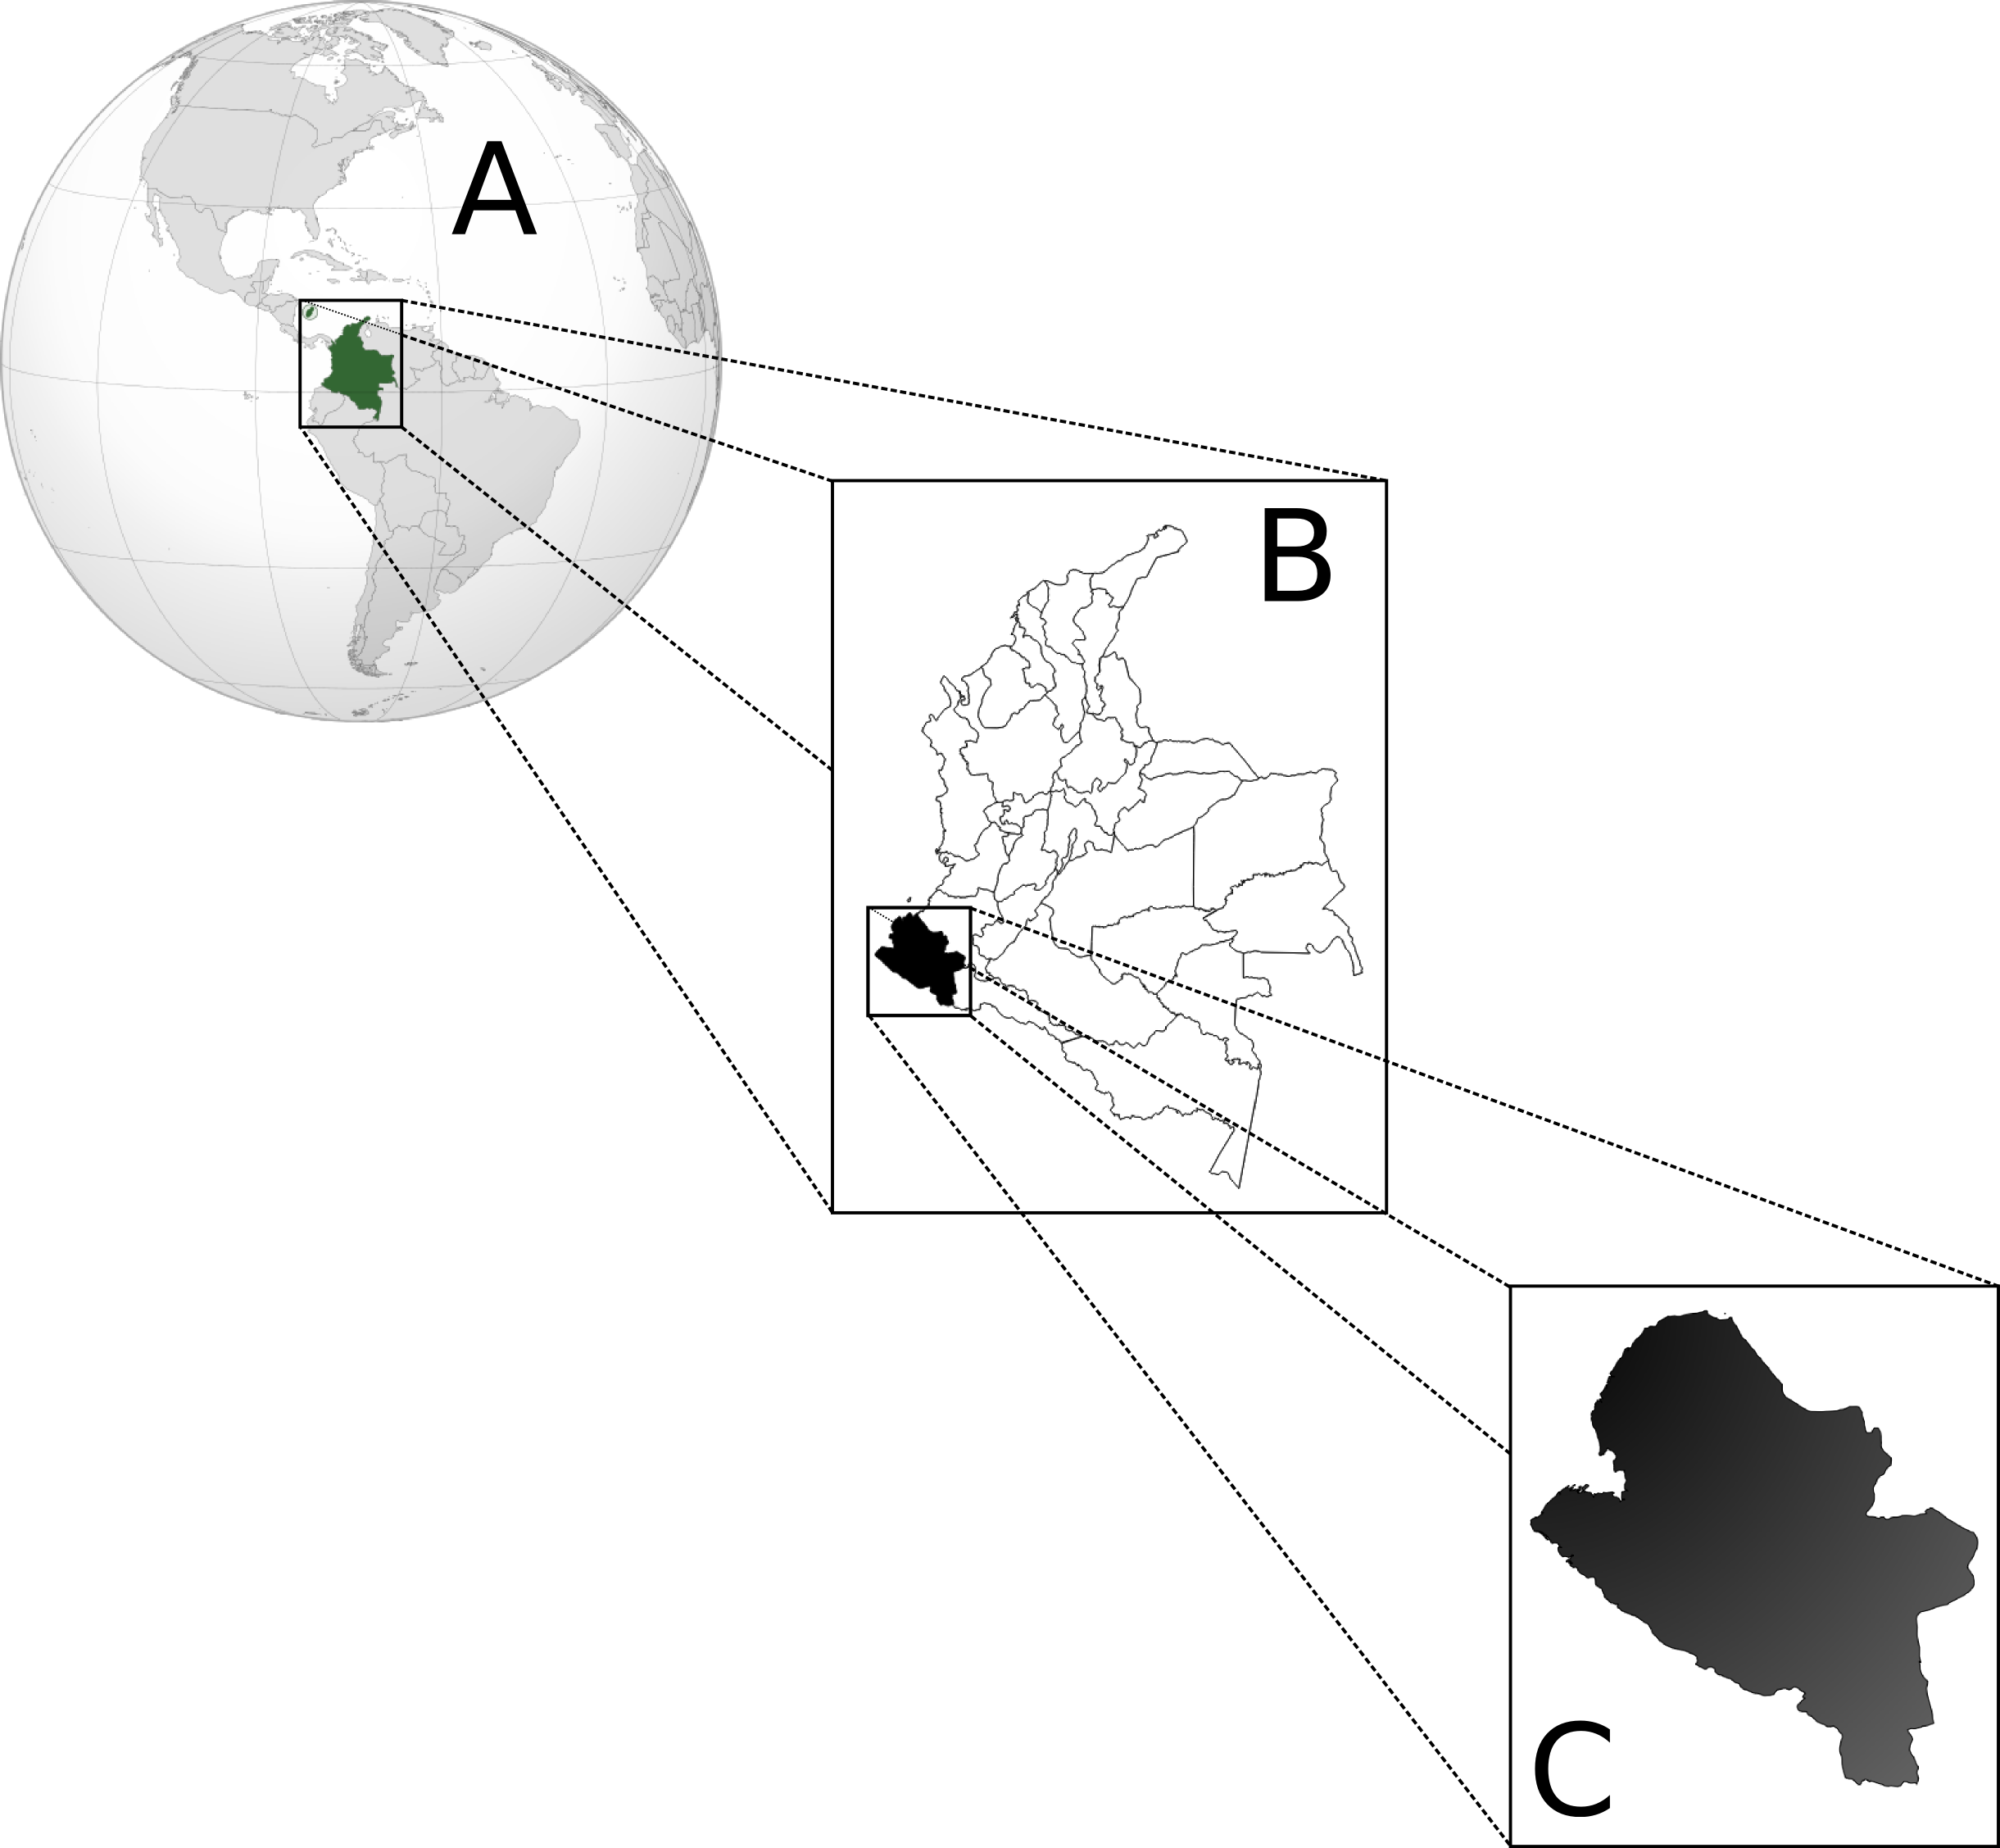
\includegraphics[width = 8cm]{locationNarino.png}
  \caption{Localización area de estudio}
  \label{fig:locationNarino}
\end{figure}